\section{问题分析}\label{sec:problem-analysis}

本题的决策始终围绕两个问题展开：干扰源还可能在哪里，下一步去哪里最合适。前者由测向与接收信息确定，后者需要权衡新增信息和行动耗时。因此，本文先建立定位区域，再据此选择测点；进入多源场景后，将寻找未知源与处理已知源一同安排，并随观测结果更新路线。

图\ref{fig:overall-framework}概括了这一思路。上层展示四问的递进关系，中层给出多源搜索的执行过程：更新定位区域，构造候选动作，比较费用，执行下一步；下层展开 D 模块的三种决策方法。位置约束用于接收与清除判断，模拟和学习模型用于估计不同动作的后续费用。


\subsection{问题一的分析}

带误差的示向度只能将源限制在一个角域内，多次测向的交集才给出定位区域。将角域写成半平面约束后，可以用凸多边形表示这一连续区域，并通过有限个顶点计算直径。题目还要求判断直径圆是否覆盖该区域，这需要单独检验，也直接关系到后续能否在某一点可靠清除干扰源。

\subsection{问题二的分析}

首测通常能较好地确定方向，却难以确定距离。第二测点适当横向偏移，可以增大交会角、缩小定位区域；偏移过大又可能失去信号，并增加移动时间。因此，先利用接收半径下界确定能够再次接收的测点范围，再在其中比较移动代价和测后定位效果。

\subsection{问题三的分析}

源数未知时，清除所有已发现源还不足以确认任务结束，需要检测站的覆盖条件判断是否遗漏。另一方面，先扫完整个场地再逐一清除容易重复移动。本文将待扫描站与已发现源合并排序，每次执行首项任务后重新规划，使未知源发现、主动定位和清除交替进行。

\subsection{问题四的分析}

定向源在接收距离内也可能因背向发射而无法被检测，因此覆盖站还需兼顾观测方位。对已发现源，则通过成对检测区分部分无信号情况，并结合正负观测约束其位置和方向。任务安排沿用第三问的滚动规划\cite{xu2021rolling}，再用蒙特卡洛 rollout 比较检测动作、用回归模型判断途中是否值得补测。

\begin{figure}[H]
\centering
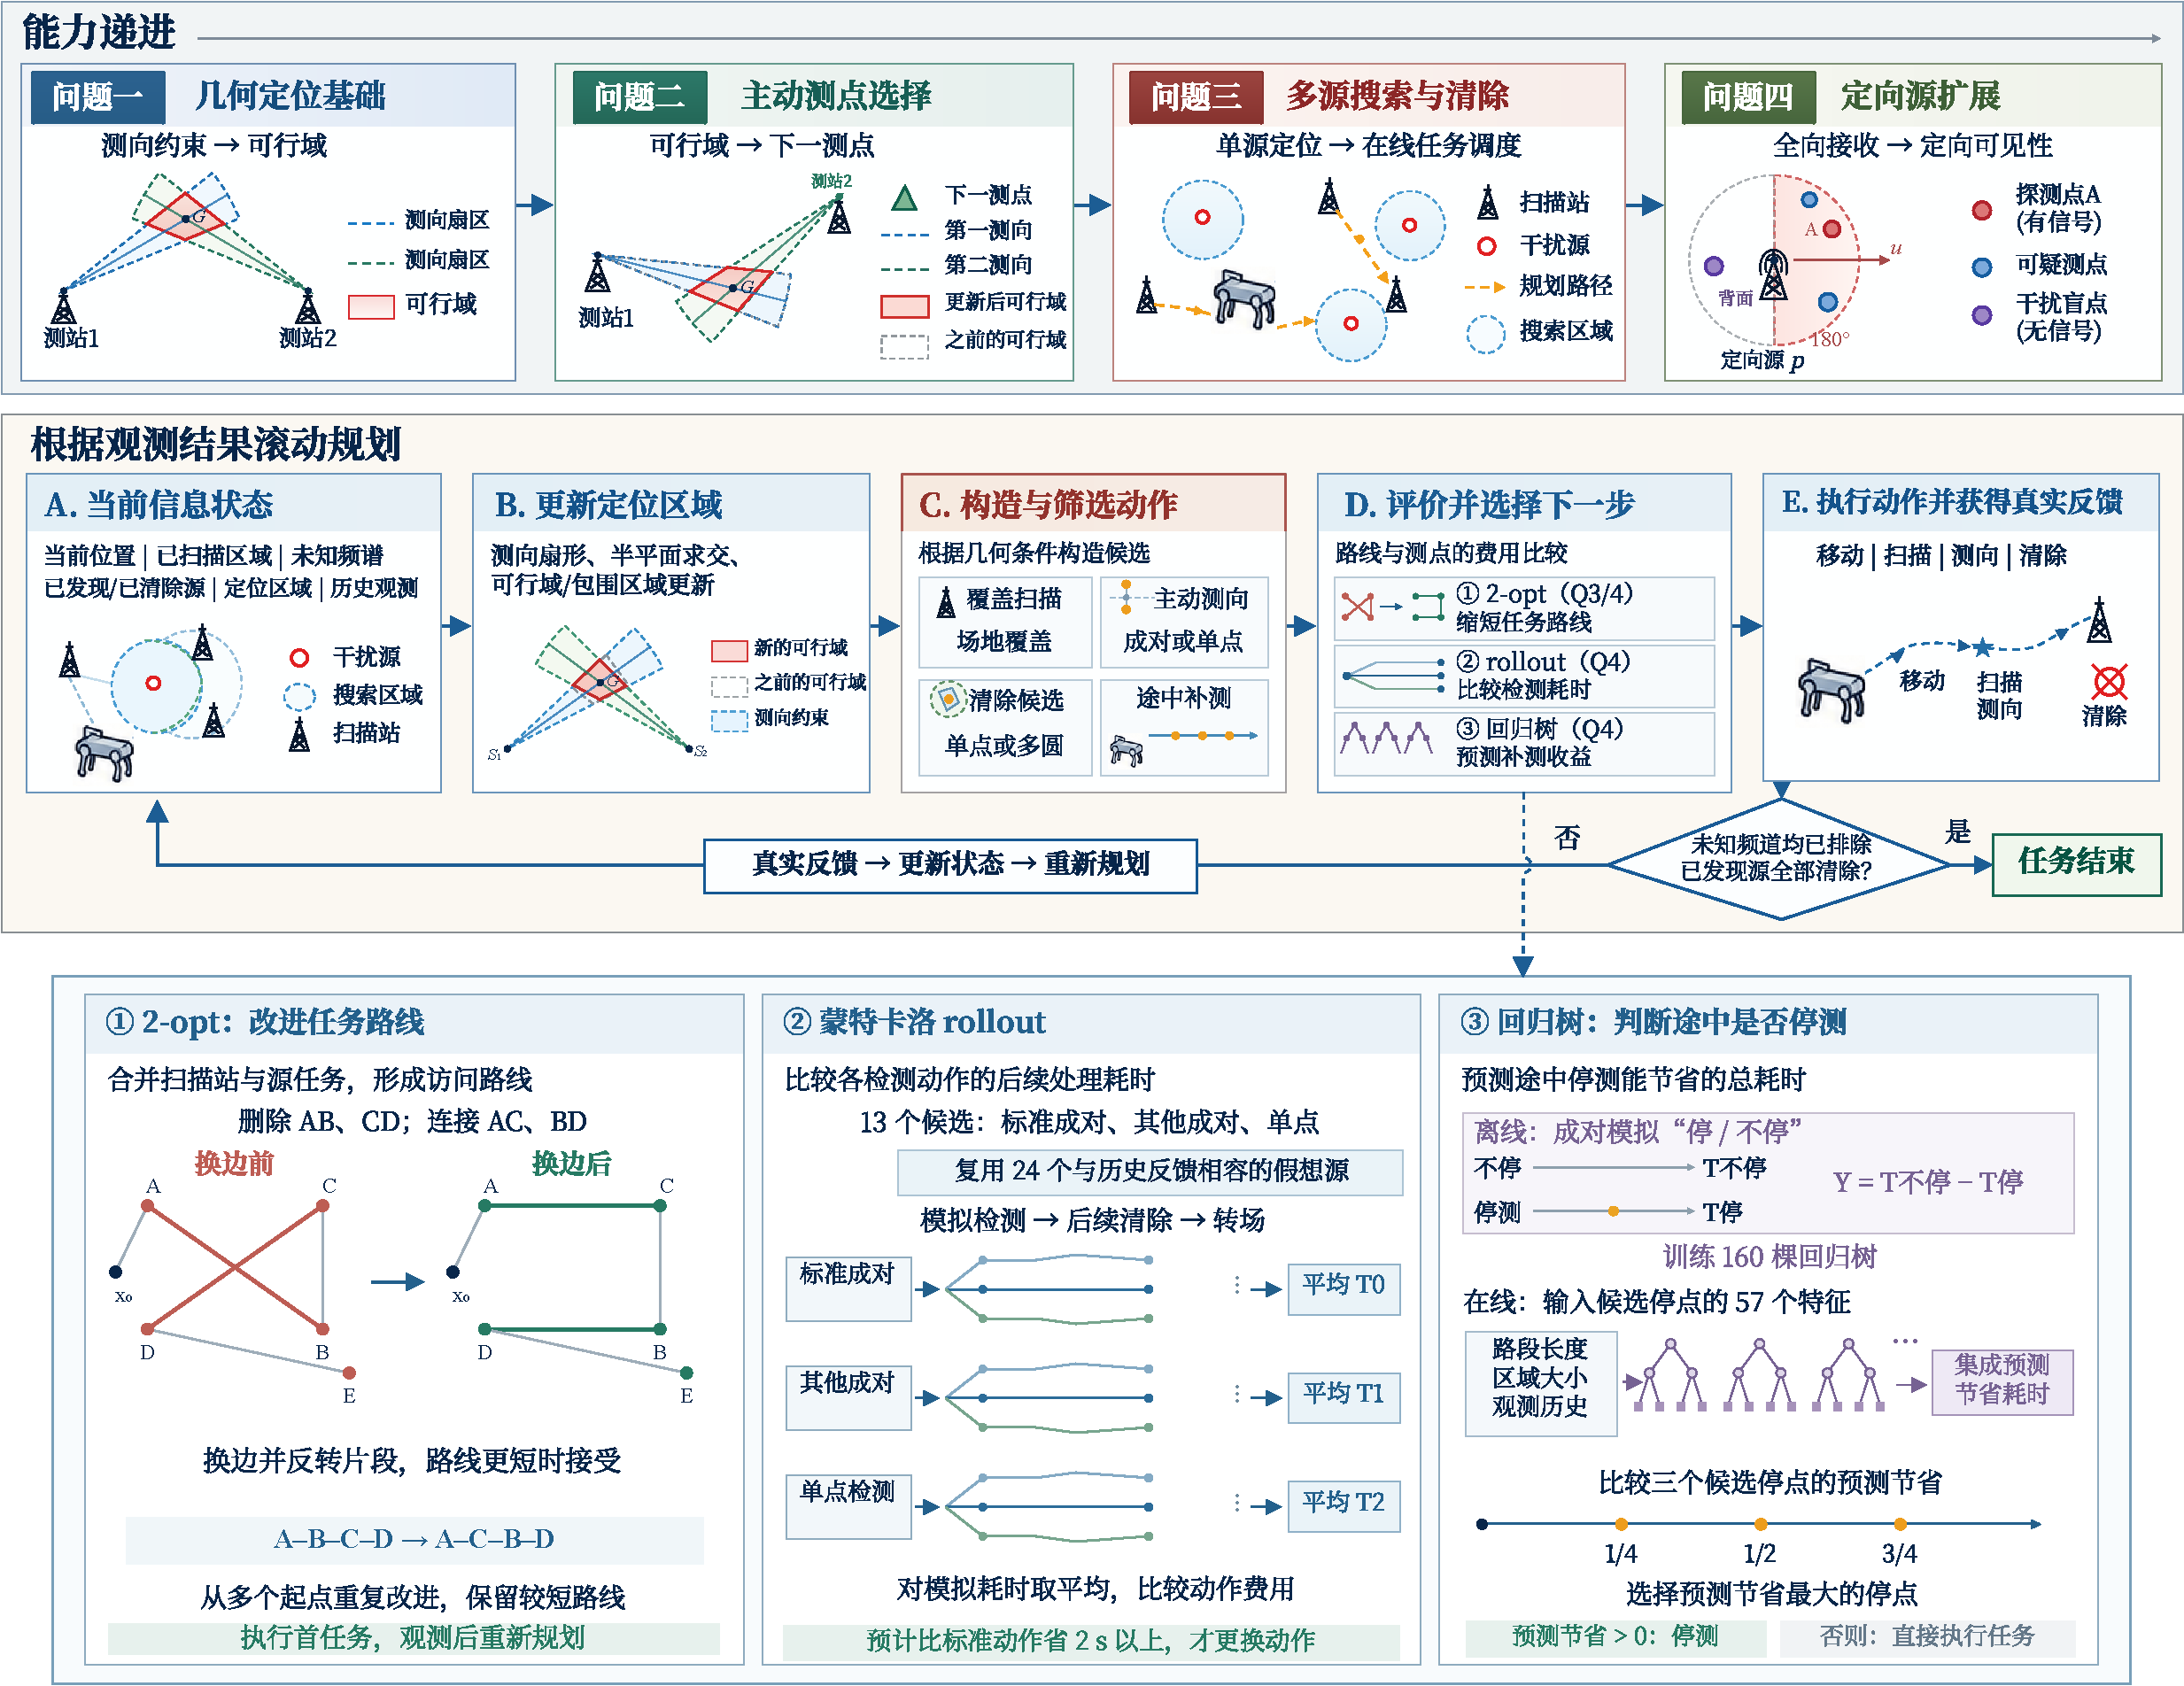
\includegraphics[width=\linewidth]{figures/overall_framework_template.pdf}
\caption{基于可行域更新与滚动规划的无线电干扰源搜索-定位-清除统一框架示意图}
\label{fig:overall-framework}
\end{figure}
